\documentclass{article}

% PACKAGES --------------------------------------------

% For layouts

\usepackage[english]{babel}
\usepackage[letterpaper,top=2cm,bottom=2cm,left=3cm,right=3cm,marginparwidth=1.75cm]{geometry}
\usepackage[skip=10pt plus1pt, indent=0pt]{parskip}
\usepackage{float}
% \usepackage[page]{appendix}


% For mathematical symbols
\usepackage{amsmath, amsfonts, amsthm, amssymb, gensymb, mathtools}


% For images, diagrams, boxed text and tables
\usepackage[usenames,dvipsnames, x11names, rgb]{xcolor}
\usepackage{graphicx}
\usepackage[]{mdframed}  % For boxed text
\usepackage{easytable}
\usepackage{tikz, pgfplots}
\pgfplotsset{compat=1.18}
% \usepackage{tikz-3dplot}
\usetikzlibrary{arrows.meta}
% \usetikzlibrary{calc}
% \usetikzlibrary{decorations.pathreplacing,calligraphy}  % Braces


% For links
\PassOptionsToPackage{hyphens}{url}\usepackage[hidelinks]{hyperref}


% For enumeration options
\usepackage{enumerate}


% Font

% \usepackage{mathptmx}  % Times New Roman
% \usepackage{bookman}  % Bookman
% \usepackage{fourier}  % Fourier
% \usepackage{tgpagella}  % TeX Gyre Pagella


% -----------------------------------------------------

% Custom commands, environments, operators and other settings

\newcommand{\abs}[1]{|#1|}

\counterwithin*{equation}{section}

\theoremstyle{definition}
\newtheorem{definition}{Definition}
\newtheorem{theorem}{Theorem}
% \newtheorem*{corollary}{Corollary}
% \newtheorem*{lemma}{Lemma}
\newtheorem{remark}{Remark}
\newtheorem{example}{Example}


% -----------------------------------------------------

% Color scheme for TikZ diagrams:
% MidnightBlue
% OliveGreen
% BrickRed
% BurntOrange
% Fuchsia

% -----------------------------------------------------

% \title{Intermediate Mathematics for Computer Science (COMP0199)}
% \author{Raphael Li}
% \date{2026}


\begin{document}
% \maketitle

% \vspace{1em}
% \hrule
% \vspace{1em}


% \tableofcontents

\section{Recap: Limits of sequences}

\begin{definition}[Limit of a sequence]
    The sequence \(u_n\) tends to or approaches a limit \(l\) if and only if for any positive real number \(\epsilon\), there is some rank \(N\) such that any term \(u_n\) of the sequence with \(n > N\) must be less than \(\epsilon\) away from \(l\), i.e.
    %
    \[\forall \epsilon > 0,\; \exists N \in \mathbb{N},\; \forall n \in \mathbb{N},\; n > N \implies\abs{u_n - l} < \epsilon\text{.}\]
\end{definition}

\begin{figure}[H]
    \centering

    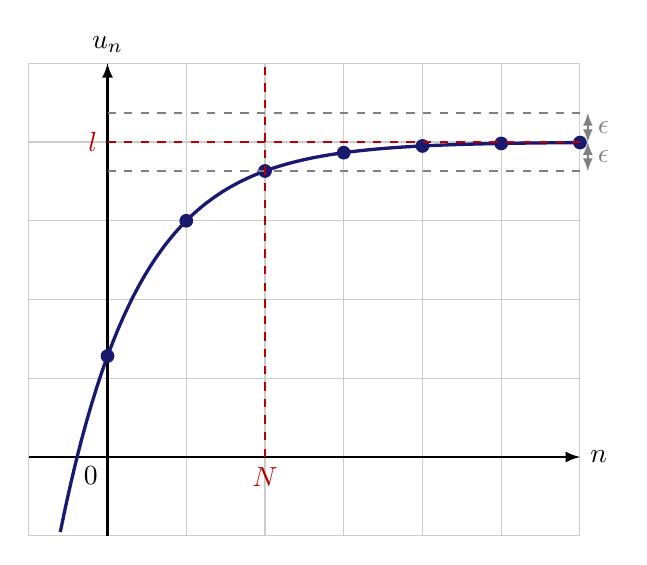
\begin{tikzpicture}
        \draw[thin,gray!40] (-1,-1) grid (6, 5);
        \draw[thick, ->, >=latex] (-1,0)--(6,0) node[right]{\(n\)};
        \draw[thick, ->, >=latex] (0,-1)--(0,5) node[above]{\(u_n\)};
        \draw (0, 0) node[below left] {0};

        \draw [MidnightBlue, very thick, domain=-0.6:6, samples=100] plot (\x, {4-2.71828^(1-\x)});

        \foreach \n in {0,...,6} {
            \filldraw[MidnightBlue] (\n,{4-2.71828^(1-\n)}) circle [radius=0.08];
        }

        \draw[gray, dashed, thick] (0, 3.63) -- (6, 3.63);
        \draw[gray, dashed, thick] (0, 4.37) -- (6, 4.37);
        \draw[BrickRed, dashed, thick] (2, 0) node[below]{\(N\)} -- (2, 5);

        \draw[BrickRed, thick, dashed] (0, 4) node[left]{\(l\)}-- (6, 4);

        \draw[gray, semithick, latex-latex, shift={(0.1, 0)}] (6, 4.37) -- (6, 4) node[pos=0.5, right] {\(\epsilon\)};

        \draw[gray, semithick, latex-latex, shift={(0.1, 0)}] (6, 4) -- (6, 3.63) node[pos=0.5, right] {\(\epsilon\)};
    \end{tikzpicture}
    
    \caption{The sequence \((u_n)\) approaches a limit \(l\).}
    \label{fig:Ch01-lim-of-seq}
\end{figure}


\begin{theorem}[Cauchy's criterion]
    A sequence of numbers \((u_n)\) is said to be Cauchy if for any positive real number \(\epsilon\), there is some rank \(N\) such that any pair of terms \(u_m\) and \(u_n\) with \(m, n \geq N\) must differ by less than \(\epsilon\), i.e.
    %
    \[\forall\epsilon > 0,\; \exists N \in \mathbb{N},\; \forall m, n \geq N,\; \abs{u_m - u_n} < \epsilon\text{.}\]
    %
    A sequence of real numbers is Cauchy if and only if it is convergent.
\end{theorem}



\newpage
\section{Sequences of functions}

\subsection{Pointwise convergence}

For each natural number \(n \in \mathbb{N}\), define a function \(f_n : A \rightarrow \mathbb{R}\), where \(A\) is their domain. We denote this sequence of functions as \((f_n)\).

\begin{example}
    For example, we can let \(A = [0, +\infty)\) and consider the sequence \(f_n(x) = x/(n+1)\). As \(n\) increases, the sequence appears to approach a zero function \(f(x) = 0\).
\end{example}

\begin{figure}[H]
    \centering

    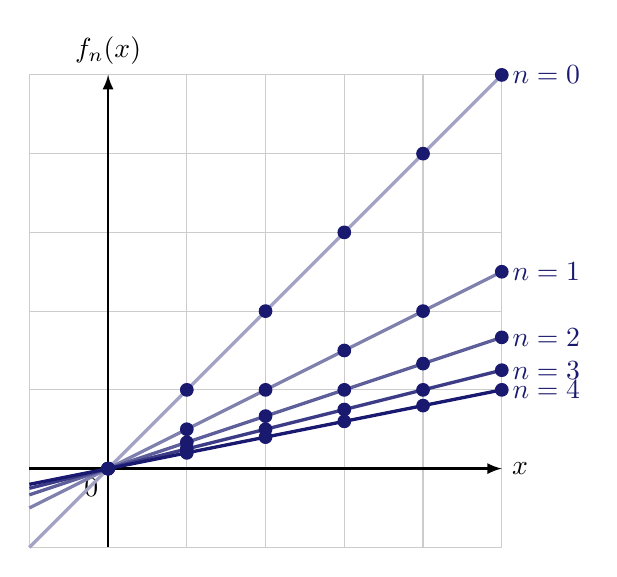
\begin{tikzpicture}
        \draw[thin,gray!40] (-1,-1) grid (5, 5);
        \draw[thick, ->, >=latex] (-1,0)--(5,0) node[right]{\(x\)};
        \draw[thick, ->, >=latex] (0,-1)--(0,5) node[above]{\(f_n(x)\)};
        \draw (0, 0) node[below left] {0};

        \draw [MidnightBlue!40, very thick, domain=-1:5] plot (\x, {\x}) node[right, MidnightBlue] {\(n=0\)};
        \draw [MidnightBlue!55, very thick, domain=-1:5] plot (\x, {\x/2}) node[right, MidnightBlue] {\(n=1\)};
        \draw [MidnightBlue!70, very thick, domain=-1:5] plot (\x, {\x/3}) node[right, MidnightBlue] {\(n=2\)};
        \draw [MidnightBlue!85, very thick, domain=-1:5] plot (\x, {\x/4}) node[right, MidnightBlue] {\(n=3\)};
        \draw [MidnightBlue!100, very thick, domain=-1:5] plot (\x, {\x/5}) node[right, MidnightBlue] {\(n=4\)};
        
        \foreach \n in {0,...,4} {
            \foreach \x in {0,...,5} {
                \filldraw[MidnightBlue] (\x,{\x/(\n+1)}) circle [radius=0.08];
            }
        }
        
    \end{tikzpicture}
    
    \caption{The sequence of functions \((f_n)\), where \(f_n(x) = x/(n+1)\), approaches a zero function \(f(x) = 0\).}
    \label{fig:Ch02-lim-of-seq-of-funcs}
\end{figure}

\begin{definition}
    For a sequence of functions \((f_n)\), if the limit \[\lim_{n\to\infty} f_n(a)\] exists for all \(a \in A\), then the sequence \((f_n)\) is said to converge pointwise to the limit
    %
    \[f(x) = \lim_{n\to\infty} f_n(a)\]
    %
    which is called the pointwise limit of the sequence.
\end{definition}

\begin{definition}
    A sequence of functions \((f_n)\) is said to be pointwise Cauchy if \((f_n(a))\) is Cauchy for all inputs \(a\).
\end{definition}

\begin{definition}
    A sequence of functions is pointwise Cauchy if and only if it is pointwise convergent.
\end{definition}

\begin{example}
    Let \(A = [0, +\infty)\) and \(f_n(x) = x/(n+1)\). The sequence converges pointwise to \(f(x) = 0\).
\end{example}
\begin{proof}
    For all \(a \in A\) we have
    %
    \[
        \lim_{n\to\infty} f_n(a) = \lim_{n\to\infty} \frac{a}{n+1} = 0\text{.} \qedhere
    \]
\end{proof}

\begin{example}
    Let \(A = [0, +\infty)\) and \(f_n(x) = 2x + \sin(nx)/n\). The sequence converges pointwise to \(f(x) = 2x\).
\end{example}
\begin{proof}
    For all \(a \in A\) we have
    %
    \[
        \lim_{n\to\infty} f_n(a) = \lim_{n\to\infty} \left(2a + \frac{\sin(na)}{n}\right) = 2a\text{.} \qedhere
    \]
\end{proof}

\begin{remark}
    Pointwise limits don't always exist. For instance, for the sequence of functions \(f_n(x) = x^n\) defined in \(x \in [0, +\infty)\), the function \(f_n(x)\)
    %
    \begin{itemize}
        \item tends to \(0\) for \(0 \leq x < 1\);
        \item tends to \(1\) for \(x = 1\); and
        \item tends to positive infinity with no finite limit for \(x > 1\),
    \end{itemize}
    %
    so this sequence has no pointwise limit.
\end{remark}

\begin{remark}
    Continuity is not necessarily preserved under pointwise convergence. Consider again the sequence of functions \(f_n(x) = x^n\), this time defined in \(x \in [0, 1]\). Although each term of the sequence is continuous, its limit
    %
    \[f(x) = \begin{cases}
        0 \text{\hspace{2em} if } 0 \leq x < 1\\
        1 \text{\hspace{2em} if } x = 1\\
    \end{cases}\]
    %
    is not continuous.
\end{remark}


\subsection{Uniform convergence}

Uniform convergence provides an alternative definition of convergence for sequences of functions, where continuity is preserved.

\begin{definition}
    A sequence of functions \((f_n)\) is said to converge uniformly to a function \(f\) on the interval \(A\) if for all positive real number \(\epsilon > 0\), there is some rank \(N\) such that any term \(f_n\) of the sequence with \(n > N\) satisfies \(\abs{f(x) - f_n(x)} < \epsilon\) for all \(x\) in \(A\), i.e.
    %
    \[\forall\epsilon > 0,\; \exists N \in \mathbb{N},\; \forall n > N,\; \forall x \in A,\; \abs{f(x) - f_n(x)} < \epsilon\text{.}\]
\end{definition}

\begin{remark}
    Note the different order of quantifiers used in pointwise and uniform convergence.
    %
    \begin{align*}
        {\color{BrickRed}\forall x \in A,}\; \forall \epsilon > 0,\; \exists N \in \mathbb{N},\; \forall n > N,\; \abs{f_n(x) - f(x)} &< \epsilon \tag{pointwise convergence}\\
        \forall \epsilon > 0,\; \exists N \in \mathbb{N},\; \forall n > N,\; {\color{BrickRed}\forall x \in A,}\; \abs{f_n(x) - f(x)} &< \epsilon \tag{uniform convergence}
    \end{align*}
\end{remark}

\begin{theorem}
    Uniform convergence implies pointwise convergence, to the same limit. However, the converse is not true.
\end{theorem}

\begin{theorem}
    If the sequence \((f_n(x))\) of continuous functions on \(A\) converges uniformly on \(A\) towards a function \(f\), then \(f\) is also continuous.
\end{theorem}



\subsection{Preservation of integrals under convergence}

For a sequence of functions, does the integral of the limit equal the limit of the integrals?

\begin{theorem}
    Given that a sequence of functions \((f_n)\) converges pointwise to a limit \(f\), the integral of the limit does not necessarily equal the limit of the integrals of terms in \((f_n)\). In other words, the equality
    %
    \[\int_a^b f(x)\, dx = \lim_{n\to\infty} \int_a^b f_n(x)\, dx\]
    %
    does not necessarily hold.
\end{theorem}
\begin{proof}
    Consider the sequence of functions defined by
    %
    \[f_n(x) = \begin{cases}
        n \text{\hspace{2em} if } 0 \leq x \leq 1/n\\
        0 \text{\hspace{2em} otherwise}
    \end{cases}\]
    %
    which converges pointwise to the zero function \(f(x) = 0\). Therefore, the integral of the limit, evaluated from \(0\) to \(1\) is zero.
    %
    \[\int_0^1 f(x)\,dx = 0\]
    %
    However, each function in the sequence has an integral of \(1\).
    %
    \begin{align*}
        \int_0^1 f_n(x)\,dx &= \int_0^{1/n} f_n(x)\,dx + \int_{1/n}^1 f_n(x)\,dx\\
        &= \int_0^{1/n} n\,dx + \int_{1/n}^1 0\,dx\\
        &= [nx]_0^{1/n}\\
        &= 1 \qedhere
    \end{align*}
\end{proof}

\begin{theorem}
    Given that a sequence of functions \((f_n)\) converges uniformly to a limit \(f\), the limit of the integrals of terms in \((f_n)\) \textbf{must exist} and be equal to the integral of the limit, i.e.
    %
    \[\int_a^b f(x)\, dx = \lim_{n\to\infty} \int_a^b f_n(x)\, dx\]
    %
\end{theorem}



\subsection{Preservation of derivatives under convergence}

\begin{theorem}
    Given that a sequence of differentiable functions \((f_n)\) converges pointwise or uniformly to a differentiable limit \(f\), the limit of the derivatives of terms in \((f_n)\) might not exist.
\end{theorem}
\begin{example}
    Let \(f_n(x) = \sin(nx)/\sqrt{n}\). The sequence \((f_n)\) converges pointwise and uniformly to the zero function. However, the limit
    %
    \[\lim_{n \to\infty} f_n'(x) = \lim_{n \to\infty} \sqrt{n}\cos(nx)\]
    %
    does not exist.
\end{example}

\begin{theorem}
    Suppose a sequence of differentiable functions \((f_n)\) converges to a function \(f\). If \((f_n')\) converges uniformly on \([a, b]\) (i.e. the limit of derivatives exists), then
    \begin{itemize}
        \item the convergence of \((f_n)\) is also uniform; and
        \item the limit of derivatives equals the derivative of the limit, with \(\lim_{n\to\infty} f_n'(x) = f'(x)\).
    \end{itemize}
\end{theorem}

\end{document}